% !TeX spellcheck = ru_RU_yo
% !TEX program = xelatex

\documentclass[pta]{../../../../scs-iam}

\begin{document}

\newgeometry{
  top=20mm,
  right=15mm,
  bottom=20mm,
  left=20mm,
  bindingoffset=0cm
}

\thispagestyle{empty}

\begin{center}
  {
    \bfseries
    {
      \subnormal
      Министерство образования и науки Российской Федерации
    } \\[-0.5em]
    {
      \scriptsize
      ФЕДЕРАЛЬНОЕ ГОСУДАРСТВЕННОЕ АВТОНОМНОЕ ОБРАЗОВАТЕЛЬНОЕ УЧРЕЖДЕНИЕ ВЫСШЕГО ОБРАЗОВАНИЯ
    } \\[-0.25em]
    {
      \subnormal
      “САНКТ-ПЕТЕРБУРГСКИЙ НАЦИОНАЛЬНЫЙ ИССЛЕДОВАТЕЛЬСКИЙ \\[-0.5em]
      УНИВЕРСИТЕТ ИНФОРМАЦИОННЫХ ТЕХНОЛОГИЙ, \\[-0.75em]
      МЕХАНИКИ И ОПТИКИ”
    } \\[1em]
  }
  \begin{minipage}{.8\textwidth}
    \titledline{\textbf{Факультет}}
    $\underset{
      \text{\scriptsize (название факультета)}
    }{
      \underline{\makebox[\remaining][c]{программной инженерии и компьютерной техники}}
    }$ \\
    \textbf{Кафедра}
    \hfill
    $\underset{
      \text{\scriptsize (название кафедры)}
    }{
      \underline{\makebox[\remaining][c]{информатики и прикладной математики}}
    }$ \\[-0.5em]
    \titledline{\textbf{Направление подготовки (специальность)}}
    \underline{\makebox[\remaining][c]{\strut 09.04.01~~}}
  \end{minipage}
\end{center}

\small

\begin{center}
  {
    \normalsize
    \textbf{О Т Ч Ё Т}
  } \\[-0.25em]
  \textbf{о}~$\underset{\text{\scriptsize (название практики)}}{\underline{\makebox[.4\textwidth][c]{производственной (НИР)}}}$~\textbf{практике}
\end{center}

{
  \parindent 0pt
  
  \textbf{Тема задания}
  \uline{<<Разработка веб-интерфейса для проведения геодезических изысканий с помощью устройств Emlid Reach и Emlid Reach RS>> \hfill} \\[-1em]
  
  \textbf{Студент}
  $\underset{
    \text{\scriptsize (Фамилия, Имя, Отчество)}
  }{
    \underline{\makebox[.65\textwidth][l]{Кузнецов Андрей Андреевич}}
  }$
  \hfill
  \textbf{Группа №}
  \underline{\makebox[.1\textwidth][c]{\strut P4215~~}} \\[-1em]
  
  \titledline{\textbf{Руководитель практики от организации}}
  $\underset{
    \text{\scriptsize (Фамилия И.О., должность и место работы)}
  }{
    \underline{\makebox[\remaining][s]{Фёдоров Е.М., ИП Николаев Д.А., руководитель от-}}
  }$
  \uline{дела разработки программного обеспечения\hfill} \\[-1em]
  
  \titledline{\textbf{Руководитель практики от университета}}
  $\underset{
    \text{\scriptsize (Фамилия И.О., должность)}
  }{
    \underline{\makebox[\remaining][l]{Исаев И.В., ассистент}}
  }$ \\[1.5em]
  
  \begin{flushright}
    \begin{minipage}{.5\textwidth}
      \titledline{\textbf{Практика пройдена с оценкой}}
      \underline{\makebox[\remaining][c]{}} \\[-1em]

      \textbf{Подписи членов комиссии}\\
      \signature\hfill
      $\underset{
        \text{\scriptsize (Фамилия И.О.)}
      }{
        \underline{\makebox[12em][s]{\strut}}
      }$ \\
      \signature\hfill
      $\underset{
        \text{\scriptsize (Фамилия И.О.)}
      }{
        \underline{\makebox[12em][s]{\strut}}
      }$ \\
      \signature\hfill
      $\underset{
        \text{\scriptsize (Фамилия И.О.)}
      }{
        \underline{\makebox[12em][s]{\strut}}
      }$ \\[0.5em]
    
      \textbf{Дата}~\datetemplate
    \end{minipage}
  \end{flushright}
}

\vfill

\begin{center}
  {
    \normalsize
    Санкт-Петербург \\
    2018 г.
  }
\end{center}

\restoregeometry
\normalsize

\clearpage

\setcounter{page}{2}

\section*{СОДЕРЖАНИЕ}
\tableofcontents

\newpage

\mysection{ОБЩИЕ СВЕДЕНИЯ}

С 5 февраля по 29 апреля 2018 года обучающийся проходил производственную практику в ИП Николаев Денис Александрович. На практику было дано задание по разработке программного модуля веб-приложения для управления ГНСС-приёмником, работающим под управлением программного обеспечения, основанного на программном комплексе высокоточного позиционирования RTKLIB.

Разрабатываемы й модуль предназначен для осуществления геодезических изысканий с помощью веб-интерфейса устройств Emlid Reach и Emlid Reach RS.

В процессе прохождения практики были изучены следующие электронные источники и литература:
\begin{dashitemize}
  \item документация программного комплекса RTKLIB;
  \item документация устройств Emlid Reach и Emlid Reach RS;
  \item техническое задание на разработку программного модуля.
\end{dashitemize}

\mysection{ХОД РАБОТЫ}

\subsection{Этап 1 -- Знакомство с платформой разработки}

В рамках данной практики платформой для разработки являлись устройства компании Emlid: ГНСС-модуль Reach и ГНСС-приёмник Reach RS. Данные устройства работают под управлением программного обеспечения, основанного на программном комплексе высокоточного позиционирования RTKLIB. Работа пользователя с данными продуктами осуществляется через веб-прило-жение, доступ к которому можно получить с помощью любого устройства, на котором установлен современный веб-браузер.

Веб-клиент рассматриваемых устройств написан с использованием языков программирования Python и JavaScript.

\newpage

Несмотря на то, что Reach и~Reach~RS созданы на базе одного и~того же вычислительного модуля и~используют одинаковые приёмники u-blox, имеется ряд существенных различий в~аппаратном обеспечении данных устройств. Различия Reach и~Reach~RS, которые необходимо учесть при создании веб-приложения, указаны в~таблице \ref{tab:reach-vs-reachrs}.

\ctable[
pos=h!,
caption={Различия Reach и~Reach~RS},
label={tab:reach-vs-reachrs}
]{|l|*{2}{>{\centering\arraybackslash}m{2.3cm}|}}{}{
  \toprule
  \multicolumn{1}{|c|}{\textbf{Техническая/функциональная особенность}} & \textbf{Reach} & \textbf{Reach~RS} \\
  \midrule
  Встроенная батарея & нет & да \\
  \midrule
  Встроенная антенна & нет & да \\
  \midrule
  Встроенное радио & нет & да \\
  \midrule
  Физическая кнопка на корпусе & нет & да \\
  \midrule
  Возможность управления фотокамерой & да & нет \\
  \bottomrule
}

\subsection{Этап 2 -- Постановка задачи}

Основной задачей производственной практики являлось создание программного компонента, необходимого для проведения геодезических изысканий с помощью вышеупомянутых ГНСС-приёмников.

Также ставится задача встраивания рассматриваемого программного модуля в существующее веб-приложение, через которое осуществляется вся работа с приёмником.

\subsubsection{Требования к модулю}
\label{subsec:survey-requirements}

Модуль должен реализовывать инструменты для проведения геодезических изысканий и~предоставлять пользователю следующие возможности:
\begin{dashitemize}
  \item создание и~удаление проектов;
  \item экспорт проектов в~различных форматах;
  \item сбор точек;
  \item просмотр данных проекта на интерактивной карте.
\end{dashitemize}

\paragraph{Создание проекта}

При создании нового проекта пользователь должен:
\begin{dashitemize}
  \item указать название проекта;
  \item указать имя автора проекта;
  \item добавить описание проекта (опционально);
  \item ввести высоту антенны по умолчанию;
  \item создать до трёх правил для автоматического сбора точек.
\end{dashitemize}

Правила для автоматического сбора точек представляют собой условия, при которых устройство автоматически будет принимать результаты усреднения координат. Параметры правил:
\begin{dashitemize}
  \item статус решения (\emph{Single} -- автономная позиция, \emph{Float} -- <<плавающее решение>> или \emph{Fix} -- <<фиксированное>> решение);
  \item минимальное время сбора (от одной секунды до одного часа);
  \item максимальное допустимое значение погрешности измерений;
  \item максимальное допустимое значение DOP (\emph{dilution of precision} с~англ. --<<снижение точности>>).
\end{dashitemize}

\paragraph{Экспорт проекта}

Экспорт проектов должен быть доступен в следующих форматах:
\begin{dashitemize}
  \item GeoJSON;
  \item ESRI Shapefile;
  \item DXF;
  \item CSV;
  \item DroneDeploy CSV.
\end{dashitemize}

\subsection{Этап 3 -- Разработка модуля}

С помощью разрабатываемого модуля приложения будет происходить основная часть работы с~устройством. Используя интерфейс модуля, пользователь может производить геодезические изыскания -- сбор точек на местности с~разделением их на проекты.

В~соответствии с~заявленными требованиями был разработан модуль приложения, основанный на сущностях и~прецедентах, описанных на рисунках \ref{fig:survey-uml-classes} и~\ref{fig:survey-uml-usecase} соответственно.

\begin{figure}[h!]
  \centering
  \setlength{\fboxsep}{5pt}
  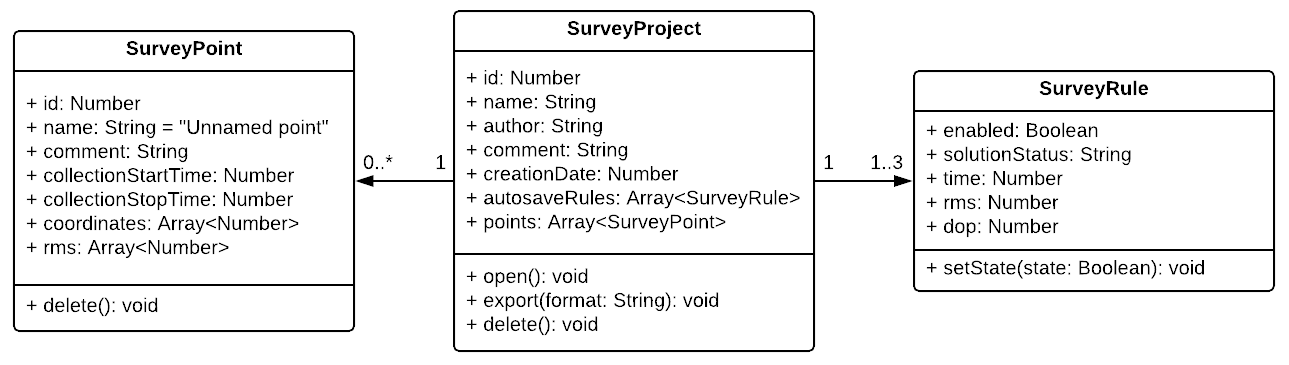
\includegraphics[width=\textwidth]{../../../../img/uml/survey_class}
  \caption{Диаграмма классов модуля}
  \label{fig:survey-uml-classes}
\end{figure}

\begin{figure}[h!]
  \centering
  \setlength{\fboxsep}{5pt}
  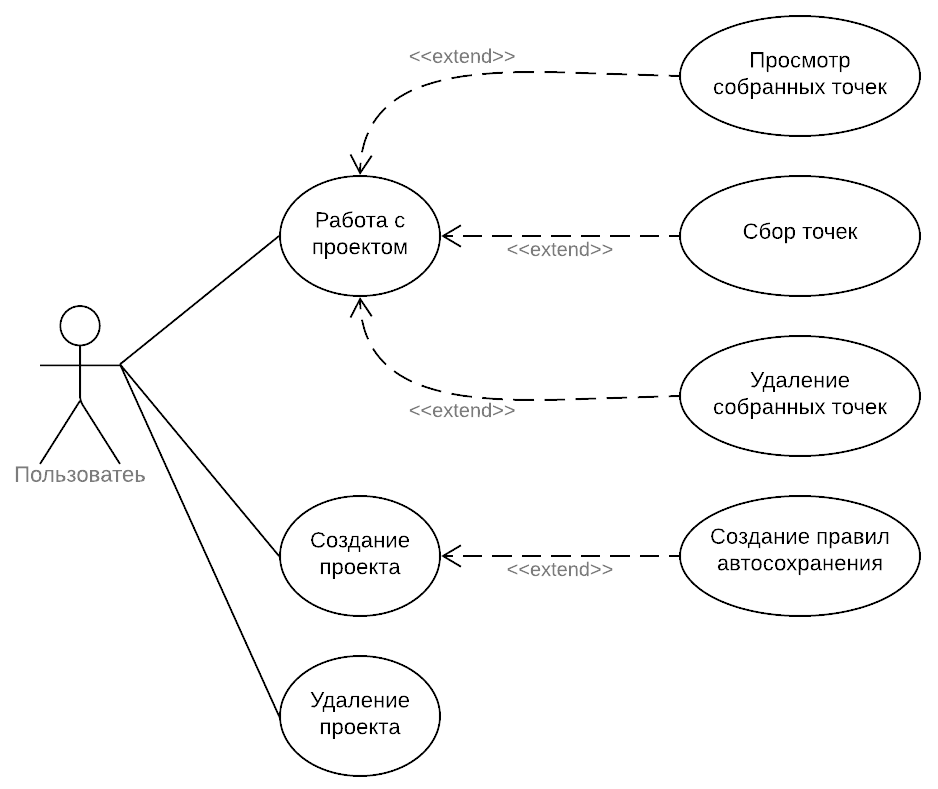
\includegraphics[width=.8\textwidth]{../../../../img/uml/survey_usecase}
  \vspace*{6pt}
  \caption{Диаграмма прецедентов модуля}
  \label{fig:survey-uml-usecase}
\end{figure}

Модуль состоит из множества отдельных представлений, переключаясь между которыми, пользователь осуществляет разнообразные действия с~собранными данными. Одной из основных задач при разработке данного модуля было чёткое описание возможных состояний и~условий перехода между ними. На рисунке \ref{fig:survey-uml-state} представлена диаграмма состояний модуля.

На данный момент рассматриваемый модуль предоставляет пользователю инструменты только для сбора точек и их организации (см. рис.~\ref{fig:survey-uml-usecase}).

В~модуле содержится следующий алгоритм сбора точек:
\begin{alphitemize}
  \item Получение очередной тройки координат;
  \item Расчёт выборочного среднего (англ. \emph{sample mean}) для координат собираемой точки;
  \item \label{itm:point-averager-variance} Вычисление несмещённой оценки дисперсии (англ. \emph{unbiased sample variance}) каждой из трёх координат;
  \item Вычисление среднеквадратичной ошибки среднего арифметического (англ. \emph{root-mean-square error, RMSE}) каждой из трёх координат;
  \item Вычисление горизонтальной среднеквадратичной ошибки среднего арифметического.
\end{alphitemize}

Для вычисления значения \ref{itm:point-averager-variance} используется метод Велфорда.

\begin{figure}[hb!]
  \centering
  \setlength{\fboxsep}{5pt}
  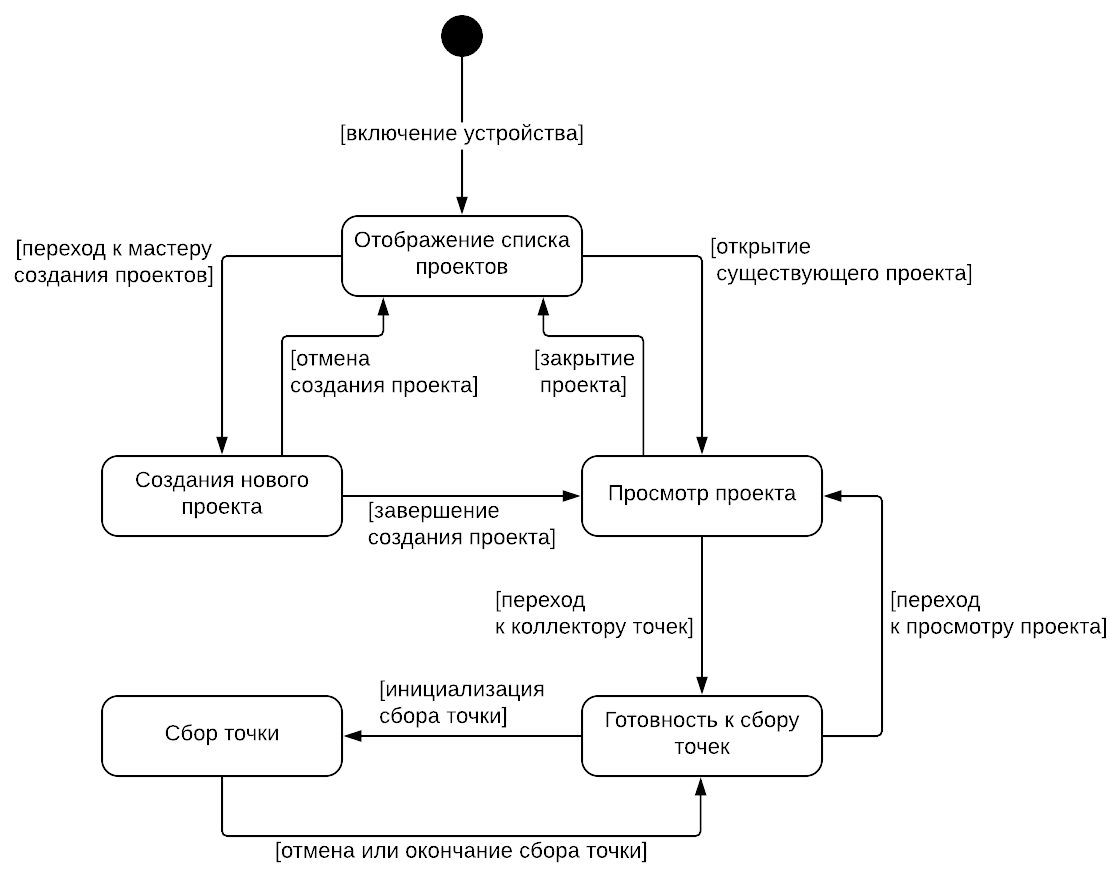
\includegraphics[width=.8\textwidth]{../../../../img/uml/survey_state}
  \caption{Диаграмма состояний модуля}
  \label{fig:survey-uml-state}
\end{figure}

\subsection{Этап 4 -- Тестирование модуля}

\subsubsection{Модульное тестирование}

В~ходе разработки исходный код приложения был покрыт модульными тестами. Для написания тестов были использованы следующие инструменты:
\begin{dashitemize}
  \item \textbf{Karma} -- утилита для запуска JavaScript-тестов;
  \item \textbf{Mocha} -- тестовый фреймворк для JavaScript-приложений;
  \item \textbf{Istanbul} -- утилита для анализа покрытия исходного кода JavaScript-приложений модульными тестами.
\end{dashitemize}

В~листинге \ref{lst:test__toggle__short} представлен пример объявления тестовых случаев (англ. \emph{test case}) и~тестовых наборов (англ. \emph{test suite}).

\lstinputlisting[
  caption={Тесты Mocha},
  label={lst:test__toggle__short}
]{../../../../src/test__toggle__short.js}

На рисунке \ref{fig:karma-output} продемонстрирован пример вывода Karma, работающей с~Istanbul.

\begin{figure}[h!]
  \centering
  \setlength{\fboxsep}{5pt}
  \fbox{
    \parbox{.9\textwidth}{
      {
        \footnotesize\ttfamily
        \$ npm run test \\
        
        ...\\
        
        Executed 148 of 154 (skipped 6) SUCCESS (6.701 secs / 5.888 secs) \\
        TOTAL: 148 SUCCESS \\
        
        ========================== Coverage summary ==========================\\
        Statements~: 58.99\% ( 1109/1880 )\\
        Branches~~~: 51.66\% ( 606/1173 )\\
        Functions~~: 47.92\% ( 115/240 )\\
        Lines~~~~~~: 59.58\% ( 1088/1826 )\\
        ======================================================================
    }}
  }
  \vspace*{6pt}
  \caption{Запуск тестов с~помощью утилиты Karma}
  \label{fig:karma-output}
\end{figure}

\subsubsection{Функциональное тестирование}

Функциональное тестирование приложения проводилось в~ручном и~автоматизированном режимах. Для автоматизации тестов были использованы язык программирования Python и~библиотека Selenuim, позволяющая автоматизировать управление веб-браузерами (см. листинг \ref{lst:pytest__short}).

Благодаря использованию тестового фреймворка pytest, предназначенного для написание тестов на Python, был автоматизирован процесс тестирования приложения в~нескольких браузерах. Вызов графического сервера Xvfb из кода Python-тестов позволил добавить возможность проверки приложения на различных разрешениях экрана.

\lstinputlisting[
  caption={Тестирование с~помощью pytest и~Selenium},
  label={lst:pytest__short}
]{../../../../src/pytest__short.py}

\subsubsection{Полевые испытания устройств}

Разработанный веб-интерфейс был протестирован при работе устройств под открытым небом. Был произведён ручной сбор точек на местности, а~также осуществлена проверка работы приложения при использовании правил автоматического сбора точек.

\subsection{Этап 5 -- Оформление пользовательской документации}

После проведения всех необходимых проверок разработанный модуль был добавлен в очередной стабильный выпуск приложения. К новому модулю была написана подробная пользовательская документация, доступная на страницах официального сайта компании Emlid.

\end{document}
